% !TEX TS-program = pdfLaTeX+shellescape
% !TEX encoding = UTF-8 Unicode

\documentclass{standalone}
\usepackage{pgfplots}
\pgfplotsset{compat=1.17}

\definecolor{tab_blue}{HTML}{1F77B4}
\definecolor{tab_orange}{HTML}{FF7F0E}
\definecolor{tab_green}{HTML}{2CA02C}
\definecolor{tab_red}{HTML}{D62728}

\begin{document}
    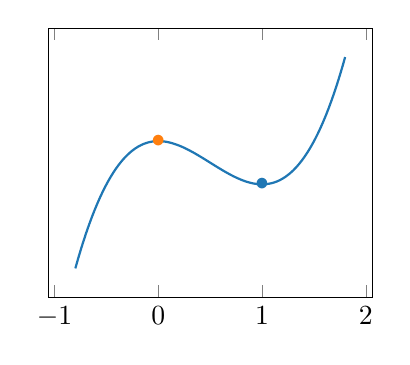
\begin{tikzpicture}[baseline]
        \begin{axis}[
            scale=0.6, % scale
            % xmin=-0.48,xmax=1.48,ymin=-0.68,ymax=1.48, % range of plot
            % legend style={at={(axis cs: 1,0)}, anchor=south east}, % position of legends
            unit vector ratio = {2, 5}, % aspect ratio
            % axis lines = box, % middle or box
            %axis x line = bottom, % top, middle, bottom, none: axis x line* = ... removes arrow heads
            %axis y line = left, % left, center, right, none: axis y line* = ... removes arrow heads
            %xlabel = {$x$}, ylabel = {$y$}, % axis labels 
            ytick = {100},
        ]
            \addplot[tab_blue, domain=-0.8:1.8, samples=100, thick] (x, x^3/3 - x^2/2);
            \node[tab_orange] at (0.0, 0.0) {$\bullet$};
            \node[tab_blue] at (1.0, -1/6) {$\bullet$};
            % \addplot3[red, thick, domain=90:300, samples=60, samples y=1]({0.8*sin(x)}, {0.8*cos(x)}, {0});
            % \addplot3[red, variable=\t, samples=7, samples y=1, domain=110:300, -latex, quiver={u={cos(t)}, v={-sin(t)}, scale arrows=0.01}]({0.8*sin(t)}, {0.8*cos(t)}, {0});
        \end{axis}
    \end{tikzpicture}
\end{document}